\section{Experimental Results}\label{sec:pcresults}
In January 2015, the authors requested from a cave exploration team in Mexico to acquire sample footage using a Dual Hero stereo camera from GoPro during a dive at an already explored cave. The selected cave is part of the Sistema Camilo, the 11th longest submerged cave system in the world, located at Quintana Roo, Yucatan peninsula, Mexico. The camera was mounted on a DPV and the video\hyp light was carried in different configurations in order to demonstrate alternative lighting schemes.

\paragraph*{Camera Calibration}As mentioned above, the stereo camera used utilizes a recording mode termed superview, which stretches the image in order to produce more aesthetically pleasing videos. Post\hyp processing all the calibration footage collected, error analysis showed, as expected, the error to slightly increase with distance; see Fig. \ref{fig:calError}. 

\begin{figure}[h]
	\begin{center}
		\leavevmode
		\hspace*{-.2cm}\begin{tabular}{cc}
			\subfloat[]{\fbox{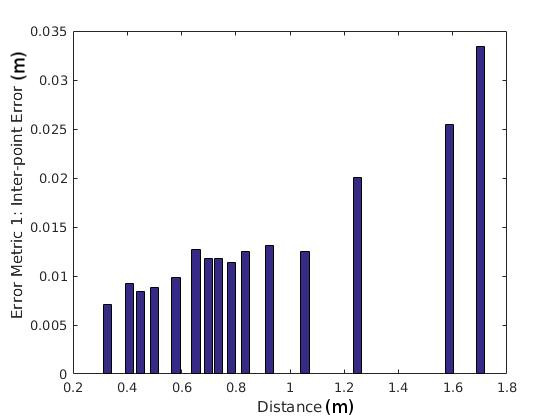
\includegraphics[width=0.47\textwidth]{./figures/error_metric1_edit.jpg}\label{fig:errMetric1}}}&
			\subfloat[]{\fbox{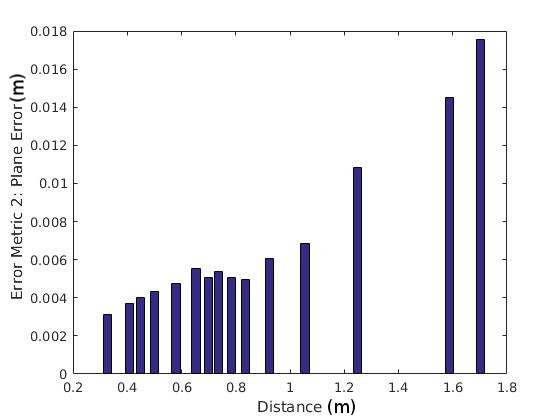
\includegraphics[width=0.47\textwidth]{./figures/error_metric2_edit.jpg}\label{fig:errMetric2}}}
		\end{tabular}
		\caption{\ref{fig:errMetric1} Average error of the inter-point distance of the target;  \ref{fig:errMetric2} Average error of the reconstructed points from the best plane fitting 3\hyp D points of the checkerboard. The results were from 4,000 images of the calibration target presented to the stereo camera underwater.}
		\label{fig:calError}
	\end{center}
\end{figure}

\paragraph*{Stereo Reconstruction}Figure \ref{fig:orb2} presents the 3\hyp D reconstruction of a long video of 7 min 28 sec. The structure corresponds with the cave morphology, however it is difficult to discern in the still image. Figure \ref{fig:tenSecDense} presents the 3\hyp D reconstruction of a cave segment from a short ten seconds traversal. The left and right walls are clearly identifiable, while the floor and ceiling are occluded from the two divers that swam in the field of view. 

\begin{figure*}[ht]
	\begin{center}
		\leavevmode
		\begin{tabular}{cc}
			\subfloat[]{{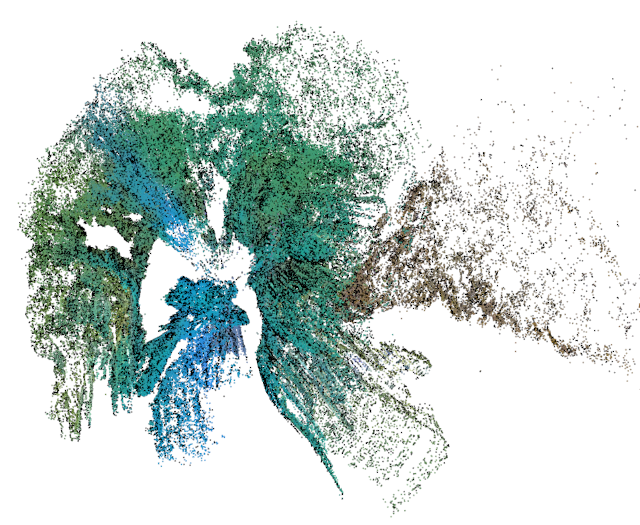
\includegraphics[width=0.75\textwidth]{./figures/dense_10sec_outsideS}\label{fig:ten1}}}\\
			\subfloat[]{{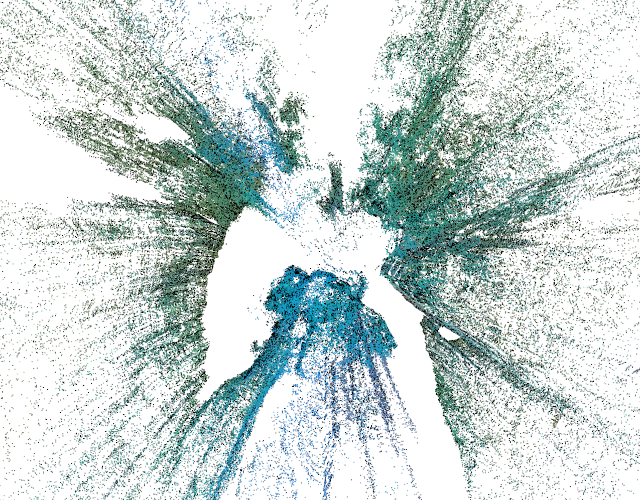
\includegraphics[width=0.75\textwidth]{./figures/dense_10sec_insideS}\label{fig:ten2}}}
		\end{tabular}
		\caption{\ref{fig:ten1} The 3\hyp D walls of the cave extracted from a short ten second traversal. \ref{fig:ten2} A second view more inside the reconstruction.}
		\label{fig:tenSecDense}
	\end{center}
\end{figure*}